\documentclass[11pt]{article}
\usepackage{graphicx}
\usepackage{hyperref}
\usepackage{natbib}

\setlength{\textwidth}{6.5in}
\setlength{\headheight}{0in}
\setlength{\textheight}{8.0in}
\setlength{\hoffset}{0in}
\setlength{\voffset}{0in}
\setlength{\oddsidemargin}{0in}
\setlength{\evensidemargin}{0in}

\title{Computational Physics: Problem Set 7}

\author{Zifeng Li}
\begin{document}
\maketitle

\section{Questions}

\subsection{Question 1}
The results are shown below:

Scipy method:  0.300000000023735

Manual implementation:  0.2999999986806734

The results are close enough to suggest that the manual method is working.

\subsection{Question 2}
The resulted graph is shown below. For the minimization method, I used scipy.optimize.
The plot shows the logistic regression model overlaid on the survey data. The curve represents the probability of recognizing the phrase as a function of age, according to the logistic model with the parameters estimated. The scatter points represent the individual responses from the survey data.
This result indicates that the older respondents are the more likely that they recognize the phrase, which makes logical sense as the phrase appears in older generation.

\begin{figure}[b!]
\centering
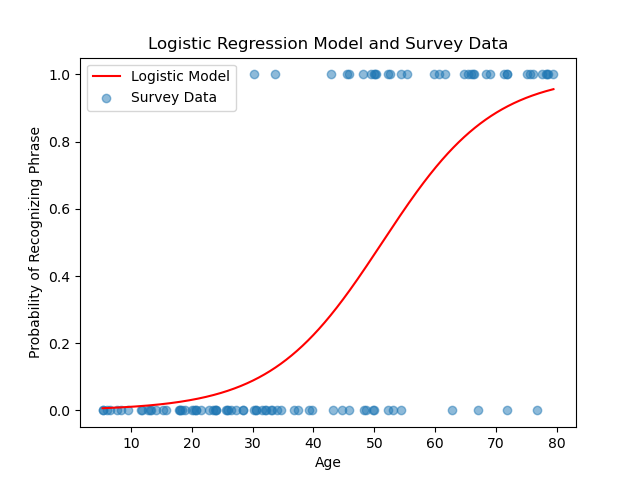
\includegraphics[width=0.95\textwidth]{Logistic Regression Model and Survey Data.png}
\end{figure}


\end{document}
